
% These are two sections that used to form the proposal:
%
% 1) ''Chap 3. Contributions'' summarize contents of oopsla '21 paper
% Most likely, not neded, because the whole paper will go in the thesis.
% But it may have some fixes from the proposal review stage. Those fixes
% could be backported to the thesis.
%
% 2) ''Chap 4. Plan of Work'' couple sentences about the STS part. Those
% sentences could be taked as inspiration.
%



% ****************************************************************************************
%              Chap. 3: Contributions
% ****************************************************************************************


\chapter{Contributions}%
\label{chap-contrib}

In my research so far, I have addressed the first two of the three tasks
declared in \secref{chap-problem} (Research Problem). First, I performed an
assessment of type stability in the wild by evaluating a corpus of Julia programs.
%
I then built a formal model of a JIT performing the key Julia optimization
(devirtualization) for type-stable code and proved its correctness. These
results are published in OOPSLA '21~\cite{Pelenitsyn21} and summarized below.


\section{Type Stability and Type Groundedness}%
\label{sec:ts-tg}

Consider the following Julia function:
\begin{lstlisting}[language=julia]
function foo()
    x = 1
    for i = 1:10
        x /= rand()
    end
    x
end
\end{lstlisting}
This function will always return a \c{Float64}, which is the type of \c{x} at
the end of the \c{foo} definition, regardless of the (nonexistent) inputs.
However, the manual says that it is a type stability issue nonetheless. This is
because the variable \c{x} is initialized to an \c{Int64} but then assigned a
\c{Float64} in the loop. Some versions of the compiler boxed \c{x} as it could
hold two different types; of course, in this example, one level of loop
unrolling would alleviate the performance issue, but in general, imprecise types
limit compiler optimizations. Conveniently, the \c{code_warntype} macro
introduced in \secref{sec:stability} will highlight imprecise types for
\emph{all} intermediate variables. Furthermore, the documentation states that
\begin{itquote}
  [t]his serves as a warning of potential type instability
\end{itquote}

Effectively, there are two competing, type-related properties of function
bodies. To address this confusion, I define two distinct terms:
\begin{itemize}
  \item \emph{type stability} is when a function's return type depends only on
    its argument types, and
  \item \emph{type groundedness} is when every variable's type depends
    only on the argument types.
\end{itemize}
Although type stability is strictly weaker than type groundedness,
my work in~\cite{Pelenitsyn21} establishes the connection between the two and
explains the role of each notion in optimizations. Type
groundedness, is useful for performance of the function itself, as it implies
that unboxing, devirtualization, and inlining can occur. The former, type
stability, allows the function to be used efficiently by other functions:
namely, type-grounded functions may call a function that is only type stable but
not grounded. For brevity, when the context is clear, I will refer to type
stability and type groundedness as stability and groundedness in what follows.

\section{Empirical Assessment of Type Stability}\label{sec:empirical}

Anecdotal evidence suggests that type stability is discussed in the
Julia community, but does Julia code exhibit the properties of stability
and groundedness in practice? And if so, are there any indicators correlated with
instability and ungroundedness? To find out, I ran a dynamic analysis on a
corpus of Julia packages. All the packages come from the main language registry
and are readily available via Julia's package manager; registered packages have
to pass basic sanity checks and usually have a test suite.

The main questions of this empirical assessment are:
\begin{enumerate}
\item How uniformly are type stability and groundedness spread over Julia packages?
  How much of a difference can users expect from different packages?
\item Are package developers aware of type stability?
\item Are there any predictors of stability and groundedness in the code and do
  they influence how type-stable code looks?
\end{enumerate}

\subsection{Methodology}

The main corpus under the study is the 1000 packages with the most GitHub stars
from the Julia package registry; as of the beginning of 2021, the registry
contained about 5.5K packages. The main corpus is used for an automated,
high-level, aggregate analysis. I also take the 10 most starred packages from
the corpus to perform finer-grained analysis and manual inspection. Out of the
1000 packages in the corpus, tests suits of only \goodpkgsnum succeeded on
\juliaversion, so these \goodpkgsnum comprise our final corpus. The reasons of
failures are diverse, spanning from missing dependencies to the absence of
tests, to timeout.

For every package of interest, the dynamic analysis runs the package test suite,
analyzes compiled method instances, and records information relevant to
type stability and groundedness. Namely, once a test suite runs to completion,
I query Julia's virtual machine for the current set of available method
instances, which represent instances compiled during the tests' execution.
The query typically returns
several hundreds to several thousands of instances,
which I
analyze for type stability and groundedness. As type information is not
directly available for compiled, optimized code, I retrieve the original method
of an instance and run Julia's type inferencer to obtain each register's type.
In rare cases, type inference may fail;
on our corpus, this almost never happened, with at most 5 failures per package.
With the inference results at hand, I check the concreteness of the register
typing and record a yes/no answer for both stability and groundedness. In
addition to that, several metrics are recorded for each method:
method size, the number of gotos and returns in the body, whether the method has
varargs or \c{@nospecialize} arguments, and
how polymorphic the method is, i.e. how many instances were compiled for it.
This information is then used to identify possible correlations between the
metrics and stability/groundedness.

To get a better understanding of type stability and performance, I employ
several additional tools to analyze the 10 packages. For example, I look at
their documentation, especially at the stated goals and domain of a package, and
check the Git history to see if and how type stability is mentioned in the
commits.

% \begin{table}[ht]\small
% \caption{Aggregate statistics for stability and groundedness}%
% \label{empirical:fig:all}
% \centering
% \begin{tabular}{@{}lrr@{}}
% \toprule
%           & \multicolumn{1}{c}{Stable} & \multicolumn{1}{c}{Grounded} \\ \midrule
% Mean      & 74\%                       & 57\%                         \\
% Median    & 80\%                       & 57\%                         \\
% Std. Dev. & 22\%                       & 24\%                         \\ \bottomrule
% \end{tabular}
% \end{table}

\subsection{Package-Level Analysis}

The aggregate results of the dynamic analysis for the \goodpkgsnum packages are
as follows: 74\% of method instances in an average package are stable and 57\%
grounded; median values are close to the means. The standard deviation is
noticeable (22\% and 24\% for type stability and groundedness respectively), so
even on small samples of packages, packages can significantly deviate from
the means.

A more detailed analysis of the 10 most starred packages, in alphabetical order,
is shown in Table~\ref{empirical:fig:top}. A majority of these packages have
stability numbers very close to the averages shown above, with the exception of
Knet, which has only 16\% of stable and 8\% of grounded instances.


\begin{table}[h]\small
\caption{Type stability and groundedness in 10 popular packages}%
\label{empirical:fig:top}
\centering
\begin{tabular}{@{}lrrrrrr@{}}
\toprule
\multicolumn{1}{c}{Package} & \multicolumn{1}{c}{Methods} & \multicolumn{1}{c}{Instances} & \multicolumn{1}{c}{Varargs} & \multicolumn{1}{c}{Stable} & \multicolumn{1}{c}{Grounded} \\ \midrule
{\footnotesize DifferentialEquations}       & 1355                        & 7381                          & 3\%                         & 70\%                       & 44\%                         \\
Flux                        & 381                         & 4288                          & 13\%                        & 76\%                       & 70\%                         \\
Gadfly                      & 1100                        & 4717                          & 10\%                         & 81\%                       & 58\%                         \\
Gen                         & 973                         & 2605                          & 2\%                         & 64\%                       & 43\%                         \\
Genie                       & 532                         & 1401                          & 12\%                        & 93\%                       & 78\%                         \\
IJulia                      & 39                          & 136                           & 8\%                         & 84\%                       & 60\%                         \\
JuMP                        & 2377                        & 36406                         & 7\%                        & 83\%                       & 63\%                         \\
Knet                        & 594                         & 9013                          & 7\%                         & 16\%                       & 8\%                          \\
Plots                       & 1167                        & 5377                          & 8\%                         & 74\%                       & 58\%                         \\
Pluto                       & 727                         & 2337                          & 4\%                         & 80\%                       & 66\%                         \\ \bottomrule
\end{tabular}

\end{table}


\paragraph{Type stability (non-)correlates}
One parameter that I conjectured may correlate with stability is the average
number of method instances per method (Inst/Meth column of
Table~\ref{empirical:fig:top}), as it expresses the amount of polymorphism
discovered in a package. Most of the packages compile just 2--4 instances per
method on average, but Flux, JuMP, and Knet have this metric 5--6 times higher,
with JuMP and Knet exploiting polymorphism the most, at 15.3 and 15.2
instances per method, respectively. The latter may be related to the very low type stability
index of Knet. However, the other two packages are more stable than the overall
average. Analyzing JuMP and Flux further, I order their methods by the number
of instances. In JuMP, the top 10\% of most instantiated methods are 5\% less
stable and grounded than the package average, whereas in Flux, the top 10\% have
about the same stability characteristics as on average. Overall,
method polymorphism is not clearly related to type stability.

Another dimension of polymorphism is the variable number of arguments in a
method (Varargs column of Table~\ref{empirical:fig:top}). I looked into three
packages with a higher than average (9\%) number of varargs methods in the 10
packages: Flux, Gadfly and Genie. Relative to the total number of methods, Flux has the most
varargs methods---13\%---and those methods are only 55\% stable and 44\%
grounded, which is a significant drop of 21\% and 26\% below this package's
averages. However, the other two packages have higher-than-package-average
stability rates, 82\% (Gadfly) and 99\% (Genie), with groundedness being high in
Genie, 93\%, and low in Gadfly, 38\%. Again, no general conclusion about the
relationship between varargs methods and their stability can be made.

One property that appear to correlate well with type stability in the sample is
application domain. For example, the Knet package, a type stability outlier,
serves as a communication layer for a GPU; most computations are done by calling
the CUDA API for the purpose of building deep neural networks. Thus, in this
specific domain, type stability of Julia code appears to be irrelevant. On the
other side of the stability spectrum is the 93\% stable (78\% grounded) Genie
package, which provides a web application framework. Inspecting the package's
Git history and issue tracker, I can confirm that its developers were aware of
type stability and intentional about performance.


\subsection{Method-Level Analysis}


In this section,
type stability of
individual methods is inspected
in its possible
relationship with other code properties like size, control flow (number of goto
and return statements), and polymorphism (number of compiled instances and varargs).
Our analysis consists of two steps: first, I plot histograms
showing the number of methods with particular values of properties, and second,
I manually sample some of the methods with more extreme characteristics.
% TODO: ^^ update after the rest of this subsection is fixed?

\paragraph{Graphical Analysis}\label{sssect:graphs}

I use two-dimensional histograms like those presented in
Fig.~\ref{figs:size:Pluto:main} to discover possible relationships between stability
of code and its other properties. The vertical axis measures stability (on the
left diagram) or groundedness (on the right): $1$ means that all recorded
instances of a method are stable/grounded, and $0$ means that none of them are.
The horizontal axis measures the property of interest; in the case of
Fig.~\ref{figs:size:Pluto:main}, it is method size (actual numbers are not
important here: they are computed from Julia's internal representation of source
code). The color of an area reflects how many methods have characteristics
corresponding to that area's position on the diagram; e.g.\ in
Fig.~\ref{figs:size:Pluto:main}, the lonely yellow areas indicate that there are about
500 (400) small methods that are stable (grounded).

\begin{figure}[h]
\centering
     \begin{subfigure}[b]{0.35\textwidth}
       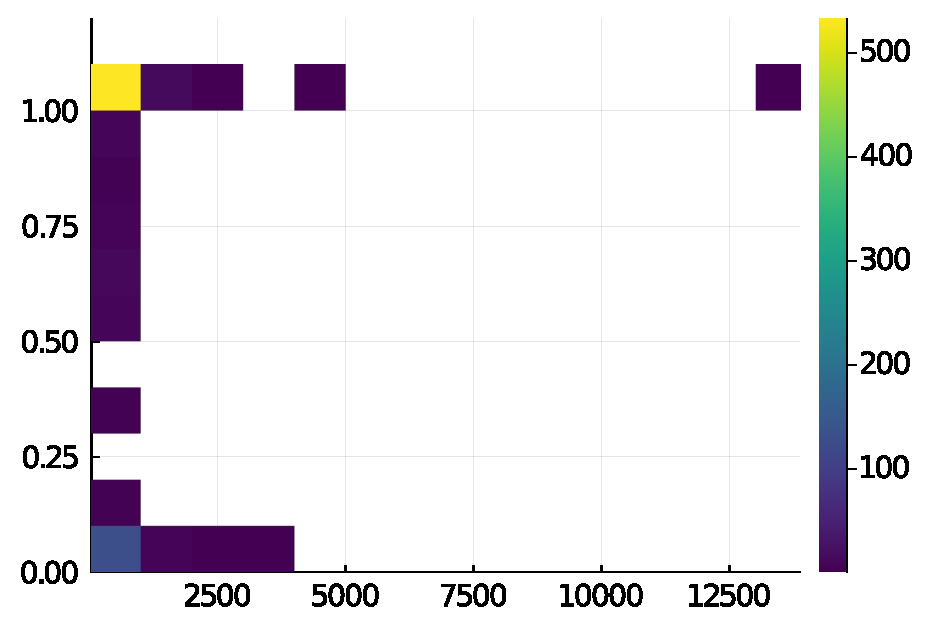
\includegraphics[width=\textwidth]{figs/Pluto-size-vs-stable.pdf}
     \end{subfigure}
     \ \ \
     \begin{subfigure}[b]{0.35\textwidth}
       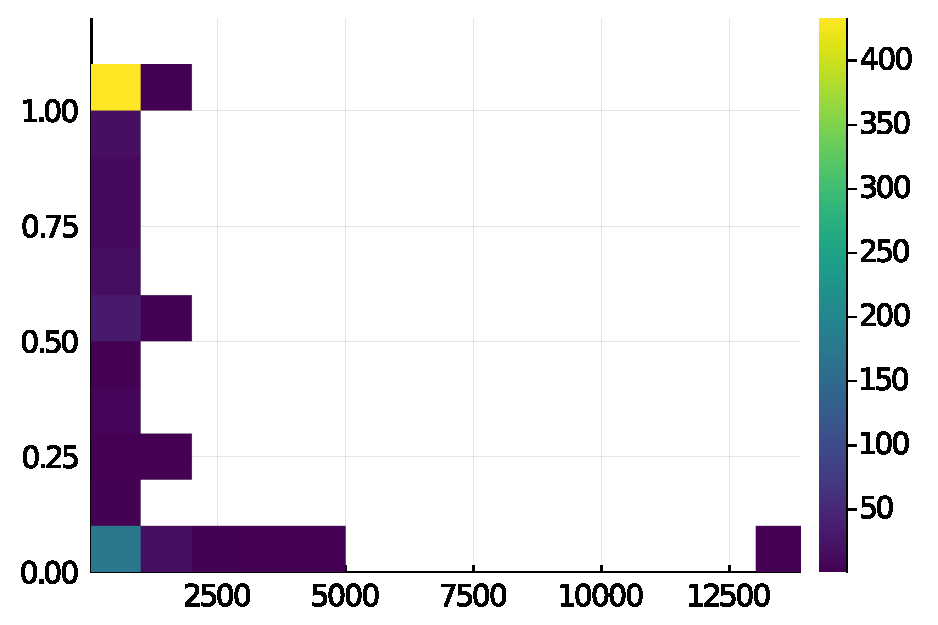
\includegraphics[width=\textwidth]{figs/Pluto-size-vs-grounded.pdf}
     \end{subfigure}
\caption{Stability (left, OY axis) and groundedness (right, OY) by method size (OX) in Pluto}%
\label{figs:size:Pluto:main}
\end{figure}

The graphs for all of the 10 packages listed in
Table~\ref{empirical:fig:top} are genertaed for all combinations of the properties of
interest\PAPERVERSIONINLINE{~\cite{oopsla21jules:arx}}{; the graphs are provided in \appref{sec:app}}.
Most of the graphs look very similar to the ones from
Fig.~\ref{figs:size:Pluto:main}, which depicts Pluto---a package for creating
Jupyter-\hspace{0pt}like notebooks in Julia. In the following paragraphs, we
discuss features of these graphs and highlight the discrepancies.

The first distinctive feature of the graphs is the hot area in the top-left
corner: most of the 10 packages employ many small, stable/grounded methods;
the bottom-left corner is usually the second-most hot, so a significant number
of small methods are unstable/ungrounded. For the Knet package,
these two corners are reversed; for DifferentialEquations, they are reversed
only on the groundedness plot. Both of these facts are not surprising after seeing
Table~\ref{empirical:fig:top}, but having a visual tool to discover such facts
may be useful for package developers.

The second distinctive feature of these graphs is the behavior of large,
ungrounded methods (bottom-right part of the right-hand-side graph). The
``tail'' of large methods on the groundedness graphs almost always lies below
the $1$-level; furthermore, larger methods tend to be less grounded.
However, if we switch from groundedness to stability plots, a large portion of
the tail jumps to the $1$-level. This means larger methods are unlikely to be
grounded (as expected, because of the growing number of registers), but they
still can be stable and thus efficiently used by other methods. Pluto provides a
good example of such a method: its \c{explore!} method of size 13003 (right-most
rectangle on Fig.~\ref{figs:size:Pluto:main}, 330 lines in the source code) analyzes
Julia syntax trees for scope information with a massive \c{if/else if/..} statement.
This method has a very low chance of being grounded, and it was not grounded on the
runs I analyzed. However, the method has a concrete return type annotation, so
Julia (and the programmer) can easily see that it is stable.

% %% PLZ, DO NOT DELETE THIS
% % Plots where the size axis is replaced with the number of branching or return
% % instructions have a technical difference from what we see on
% % Fig.~\ref{figs:size:Pluto:main} in that they reflect individual method instances
% % instead of methods because due to Julia's simple optimizer, which kicks i
% % when the main optimizer is turned off by our demand, instances of a method can
% % have different number of those instructions. As a consequence, all squares on
% % the histograms lie either on $1$-level or $0$-level. Otherwise, the picture is
% % similar to Fig.~\ref{figs:size:Pluto:main} in the two distinctive feature discussed
% % above.

% In the case of the number of gotos and returns, the plots are largely similar
% to the ones for method size, but they highlight one more package with low
% groundedness. Namely, the Gen package (aimed at probabilistic
% inference~\cite{JuliaGenPkgPub2019}) has the hottest area in the bottom-left
% corner, contrary to the first general property we identified for the size-based
% plots. Recall (Tables \ref{empirical:fig:all} and \ref{empirical:fig:top}) that
% Gen's groundedness is 14\% less than the average on the whole corpus of
% \goodpkgsnum packages.

\paragraph{Manual Inspection}

To better understand the space of stable methods,
I perform a qualitative analysis of a sample of stable methods that
have either large sizes or many instances.

Many large methods have one common
feature: they often have a return type ascription on the method header of
the form:
\begin{lstlisting}[language=julia]
function f(...) :: Int
  ...
end
\end{lstlisting}
These ascriptions are a relatively new tool in Julia, and they are used only
occasionally, in our experience. An ascription makes the Julia compiler insert implicit
conversions on all return paths of the method. Conversions are user extendable:
if the user defines type \c{A}, they can also add methods of a special
function \c{convert} for conversion to \c{A}. This function will be called
when the compiler expects \c{A} but infers a different type, for example,
if the method returns \c{B}.
If the method returns \c{A}, however, then \c{convert} is a no-op.

Type ascriptions may be added simply as documentation, but they can also
be used to turn type instability into a run-time error:
if the ascribed type is concrete and a necessary conversion is not available,
the method will fail. This provides a useful, if
unexpected, way to assure that a large method never becomes unstable.

While about 85\% of type-stable methods in the top 10 packages are uninteresting
in that they always return the same type, sampling the rest illuminates
a clear pattern: the methods resemble what we
are used to see in statically typed languages with parametric polymorphism.
% Below is a list of categories that we identify in this family.
Here are the subcategories identified in this group of methods.

\begin{itemize}
\item
  Various forms of the identity function---a surprisingly popular function that
  packages keep reinventing. In an impure language, such as Julia, an identity
  function can produce various side effects.
  For example, the Genie package adds a caching effect to
  its variant of the identity function called \c{secret_token!}.

\item Container manipulations for various kinds of containers, such as arrays,
  trees, or tuples. For instance, the Flux package defines the
  \c{extraChain} function that maps a tuple of functions by applying
  them to a given argument.

\item
  Smart constructors for user-defined polymorphic structures. For example, the
  \c{build_constraint} convenience function from JuMP creates an instance of the
  \c{VectorConstraint} structure with three fields, each of which is polymorphic.

\item
  Type computations---an unusually wide category for a dynamically typed
  language. For instance, the Gen package defines a type that represents generative
  functions in probabilistic programming; the type has two type parameters, for
  argument and for return type of the function; in order to extract those type
  arguments (and return them as objects) Gen defines two simple polymorphic functions.

\end{itemize}

\subsection{Main Results}

My analysis shows that a Julia user can expect mostly stable (74\%) and
somewhat grounded (57\%) code in widely used Julia packages. If the authors
are intentional about performance and stability, as demonstrated by the Genie
package, those numbers can be much higher. Although my sample of packages is
too small to draw strong conclusions, several factors can be
used by a Julia programmer to pinpoint potential sources of instability in their
package. For example, in some cases, varargs methods might indicate instability.
Large methods, especially ones with heavy control flow,
tend to not be type grounded but often are stable; in particular,
if they always return the same concrete type.
Finally, although highly polymorphic methods are neither stable nor unstable
in general, code written in the style of parametric polymorphism
often suggests type stability.

My dynamic analysis and visualization code is written in Julia (and some bash
code), and relies on the vanilla Julia implementation. Thus, it can be employed
by package developers to study type instability in their code, as well as check
for regressions.


\section{Formalizing Type Stability: Jules}%
\label{sec:jules}


Formal reasoning about type stability and groundedness is based on
\jules, an abstract machine that provides an idealized version of
Julia's intermediate representation (IR) and compilation model.
\jules captures the just-in-time (JIT) compilation process that (1) specializes methods
for concrete argument types as the program executes, and (2) replaces dynamically
dispatched calls with direct method invocations when \emph{type inference}
is able to get precise information about the argument types.
% Note that type inference algorithm directly affects
% type stability and groundedness of code, and thus the ability of the JIT compiler
% to optimize it. While Julia's actual type inference algorithm
% is quite complex, its implementation is not relevant for understanding
% our properties of interest; thus, \jules abstracts over type inference
% and uses it as a black box.

\begin{figure}[!h]
  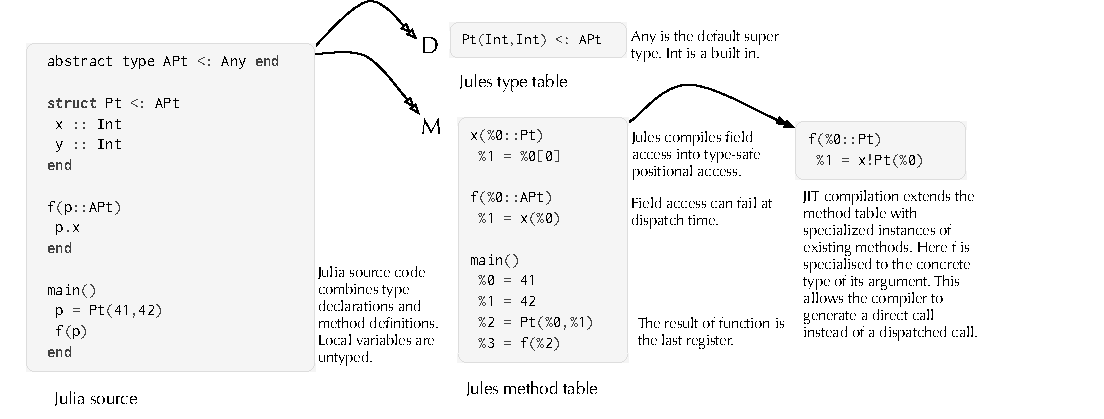
\includegraphics[width=1.1\columnwidth]{figs/compile.pdf}
  \caption{Compilation from Julia to \jules}\label{comp}
\end{figure}

Fig.~\ref{comp} illustrates the relationship between Julia source code, the
\jules intermediate representation, and the result of compilation. I do not model
the translation from the source to \jules, and simply assume that the front-end
generates well-formed \jules code.\footnote{The front-end does not devirtualize
function calls, as Julia programmers do not have the ability to write direct
method invocations in the source.} A \jules program consists of an immutable \emph{type
table}~\tytbl and a \emph{method table}~\mtbl; the method table can be incrementally extended
with method instances that are compiled by the just-in-time compiler.

The source program of Fig.~\ref{comp} defines two types, the concrete \c{Pt} and
its parent, the abstract type \c{APt}, as well as two methods, \c{f} and
\c{main}. When translated to \jules, \c{Pt} is added to the type table along
with its supertype \c{APt}. Similarly, the methods \c{main} and \c{f} are added
to the \jules method table, along with accessors for the fields of \c{Pt}, with
bodies translated to the \jules intermediate representation.

The \jules IR is similar to static single assignment form. Each statement can
access values in registers, and saves its result into a new, consecutively
numbered, register. Statements can perform a dispatched call \c{f(\%2)}, direct
call \c{x\!Pt(\%0)}, conditional assignment (not shown), and a number of other
operations. The IR is untyped, but the translation from Julia is type sound. In
particular, type soundness guarantees that only dispatch errors can occur at run
time. For example, compilation will produce only well-formed field accesses such
as the one in \c{x(\%0::Pt)}, but a dispatched call \c{x(\%0)} in \c{f} could
fail if \c{f} was called with a struct that did not have an \c{x} field. In
order to perform this translation, \jules uses type inference to determine the
types of the program's registers. I abstract over this type inference mechanism
and only specify that it produces sound (with respect to our dynamic semantics)
results. %, but do not describe its operation.

Execution in \jules occurs between \emph{configurations} consisting of both
a stack of \emph{frames} \frm (representing the current execution state)
and a \emph{method table} \mtbl (consisting of original methods and specialized
instances), denoted $\config{\frm}{\mtbl}$. A configuration
$\config{\frm}{\mtbl}$ evolves to a new configuration
$\config{\frm'}{\mtbl'}$ by stepping $\config\frm\mtbl \step
\config{\frm'}{\mtbl'}$; every step processes the top instruction in $\frm$
and possibly compiles new method instances into $\mtbl'$.
% Notably, due to the
% so-called world-age mechanism~\cite{oopsla20a} which restricts the effect
% of \c{eval}, source methods are fixed from the
% perspective of compilation; only compiled instances changes.

\subsection{Syntax}

The syntax of \jules methods is defined in~\figref{syntax}.
There are two key
notational devices. First, sequences are denoted \ol{\,\cdot\,}; thus, \ol\ty
stands for types $\ty_0\dots\ty_n$, \ol{\v\k} for registers $\v\k_0\dots\v\k_n$,
and \ol\st for instructions $\st_0\dots\st_n$. An empty sequence is written
\emp. Second, indexing is denoted $[\cdot]$; \idx{\ol\ty}\k is the $k$-th type
in \ol\ty (starting from 0), \get\j\k is the $k$-th field of \v\j, and
\idx\mtbl{\msig\m{\ol\ty}} indexes \mtbl by method signature where \m denotes
method name and \ol\ty denotes argument types.

\begin{figure}[!h]\footnotesize
% \begin{tabular}{lcl}
\begin{tabular}{lll}
\ty &::=& \Ty  \\
    & | & \aty \\
\\
  \tytbl &::=& $\left(\ \ \msig\Ty{\ol\ty} ~<:~ \aty \ \ \right)\!*$
\\
\\
  \mtbl  &::=& $\left(\ \ \langle \meth\m{\ol{\ty'}}{\ol{\v\j}}\ol\st,\ \ol{\ty}\rangle \ \ \right)\!*$
\\
\end{tabular}
% &\;&
~%
\begin{tabular}{ll@{~}ll}
\st &::=& & instruction\\
    & | & $\ass\i\p$                                       &\it int. assignment\\
    & | & $\ass\i{\v\j}$                                   &\it reg. transfer\\
    & | & $\ass\i{\construct\Ty{\ol{\v\k}}}$               &\it allocation\\
    & | & $\ass\i{\get\j\k}$                               &\it field access\\
    & | & $\cond\i\j{\call\m{\ol{\v\k}}}{\v\l}$            &\it dispatched call\\
    & | & $\cond\i\j{\direct\m{\ol{\Ty}}{\ol{\v\k}}}{\v\l}$&\it direct call\\
    & \multicolumn{2}{l}{$i \in \mathbb{N},\ \p \in \mathbb{Z}$}                 &  \\
\end{tabular}
% \end{tabular}
\caption{Syntax of \jules}\label{syntax}
\end{figure}

Types \ty live in the immutable type table \tytbl, which contains both concrete
(\Ty) and abstract (\aty) types. Each type table entry is of the form
$\msig{\Ty}{\ol\ty} <: \aty$, introducing concrete type $\Ty$, with fields of
types $\ol\ty$, along with the single supertype $\aty$. Two predefined types are
the concrete integer type \int, and the universal abstract supertype \any.

Method tables \mtbl contain method definitions of two sorts:
first, original methods that come from source code;
second, method instances compiled from original methods.
To distinguish between the two sorts, \jules stores the type signature of the
original method in every table entry.
Thus, table entry
$\langle\meth\m{\ol{\ty'}}{\ol{\v\j}}\ol\st,\ \ol{\ty}\rangle$ describes a
method \m with parameter types $\ol{\ty'}$ and the body comprised of
instructions $\ol\st$; type signature \ol{\ty} points to the original method.
If \ol\ty is equal to \ol{\ty'}, the entry defines an original method,
and \ol{\st} cannot contain direct calls.
Otherwise, \ol{\ty'}
denotes some concrete types~\ol\Ty, and the entry defines a
method instance compiled from \msig\m{\ol\ty}, specialized for concrete argument
types $\ol\Ty <: \ol\ty$.
Method table may contain multiple method definitions with the same name,
but they have to have distinct type signatures.

Method bodies consist of instructions \ol{\st}. An instruction $\v{\i}
\leftarrow \text{\c{op}}$ consists of an operation \c{op} whose result is
assigned to register $\v\i$. An instruction can assign from a primitive integer
\p, another register \v\j, a newly created struct $\construct\Ty{\ol{\v\k}}$
of type \Ty with field values $\ol{\v\k}$, or the result of looking up a struct
field as $\get\j\k$. Finally, the instruction may perform a function call. Calls
can be dispatched, $\call\m{\ol{\v\k}}$, where the target method is dynamically
looked up, or they can be direct, \direct\m{\ol\Ty}{\ol{\v\k}}, where the target
method is specified. All calls are conditional: \EM{\v\j ~?~ \text{\c{call}} :
  \v\l}, to allow for recursive functions.
If the register \v\j is non-zero, then \c{call} is performed. Otherwise,
the result is the value of register \v\l. Conditional calls can be trivially
transformed into unconditional calls; in examples, this transformation is
performed implicitly.

\subsection{Dynamic Semantics}

\jules is parameterized over three components: method dispatch $\mathcal D$,
type inference $\mathcal I$, and just-in-time compilation \jit. I do not
specify how the first two work, and merely provide their interface and a set of
criteria that they must meet (in sections \ref{sec:disp} and \ref{sec:infer},
respectively). The compiler, \jit, is instantiated with either the identity
function, which gives a regular non-optimizing semantics, or an optimizing
compiler, which is defined in section~\ref{sec:comp}. The optimizing compiler
relies on type inference $\mathcal I$ to devirtualize method calls. Type
inference also ensures well-formedness of method tables. Method dispatch
$\mathcal D$ is used in operational semantics.

\begin{figure}[!t]\small
\begin{tabular}{rclcrclcrcl}
\val &::=& \p\ |\ \construct\Ty{\ol\val}
& \qquad &
\env &::=& \ol\val
& \qquad &
\frm &::=& \done\ |\ \stk{\env\ \ol\st}{\frm} \\
\end{tabular}
\begin{mathpar}
\PAPERVERSIONINLINE{}{\framebox{\configd \step \config{\frm'}{\mtbl}}\\}

\inferrule[Prim]{
  \st = \ass\i\p\\\\
  \env' = \env + \p
}{
  \config{ \stk{ \env \ \st\,\ol\st}{\frm} }{\mtbl} \step
  \config{ \stk{ \env'\ \ol\st     }{\frm} }{\mtbl}
}

\inferrule[Reg]{
  \st = \ass\i{\v\j}\\\\
   \env'=\env + \idx\env\j
}{
  \config{ \stk{ \env \ \st\,\ol\st}{\frm} }{\mtbl} \step
  \config{ \stk{ \env'\ \ol\st     }{\frm} }{\mtbl}
}

\inferrule[New]{
  \st= \ass\i{\construct\Ty{\ol{\v\k}}}\\\\
  \env'  = \env + \construct\Ty{\idx\env{\ol{k}}}
}{
  \config{ \stk{ \env \ \st\,\ol\st }{\frm} }{\mtbl} \step
  \config{ \stk{ \env'\ \ol\st      }{\frm} }{\mtbl}
}
\\

\inferrule[Field]{
  \st= \ass\i{\get\j\k}\\\\
  \val = \idx\env\j \and
  \env' = \env + \idx\val\k
}{
  \config{ \stk{ \env \ \st\,\ol\st }{\frm} }{\mtbl} \step
  \config{ \stk{ \env'\ \ol\st      }{\frm} }{\mtbl}
}

\inferrule[False1]{
  \st= \cond\i\j{\call\m{\ol{\v k}}}{\v\l}\\\\
  0 = \idx\env\j \and
  \env'=\env +  \idx\env\l
}{
  \config{ \stk{ \env \ \st\,\ol\st }{\frm} }{\mtbl} \step
  \config{ \stk{ \env'\ \ol\st      }{\frm} }{\mtbl}
}

\inferrule[False2]{
  \st= \cond\i\j{\direct\m{\ol\Ty}{\ol{\v\k}}}{\v\l}\\\\
  0 = \idx\env\j \and
  \env'=\env + \idx\env\l
}{
  \config{ \stk{ \env \ \st\,\ol\st }{\frm} }{\mtbl} \step
  \config{ \stk{ \env'\ \ol\st      }{\frm} }{\mtbl}
}
\\

\inferrule[Disp]{
  \st= \cond\i\j{\call\m{\ol{\v\k}}}{\v\l}\\\\
  0 \not=\idx\env\j \and
  \ol\Ty = \typeof(\idx\env{\ol{k}}) \and
  \mtbl' = \jit(\mtbl, \m, \ol\Ty) \\\\\
  \ol{\st'} = \body(\dispatch{\mtbl'}\m{\ol\Ty}) \and
  \env' =  \idx\env{\ol{k}}
}{
  \config{                        \stk{\env\ \st\,\ol\st}{\frm}  }{\mtbl} \step
  \config{ \env'\ \stk{\ol{\st'}}{\stk{\env\ \st\,\ol\st}{\frm}} }{\mtbl'}
}

\inferrule[Direct]{
  \st= \cond\i\j{\direct\m{\ol\Ty}{\ol{\v\k}}}{\v\l}\\\\
  0 \not = \idx\env\j \\\\
  \ol{\st'} = \body(\mtbl[\msig\m{\ol\Ty}]) \and
  \env' = \idx\env{\ol{k}}
}{
  \config{                        \stk{\env\ \st\,\ol\st}{\frm}  }{\mtbl} \step
  \config{ \env'\ \stk{\ol{\st'}}{\stk{\env\ \st\,\ol\st}{\frm}} }{\mtbl}
}

\inferrule[Ret]{
  \env''=\env + \last{\env'}
}{
  \config{ \stk{\env'\ \done}{\stk{ \env  \ \st\,\ol\st }{\frm}}}{\mtbl} \step
  \config{                    \stk{ \env''\ \ol\st      }{\frm} }{\mtbl}
}
\end{mathpar}
\caption{Operational semantics of Jules}\label{sems}
\end{figure}

\paragraph{Operational Semantics}\label{sec:opsem}

Fig.~\ref{sems} gives rules for the dynamic semantics. Given a type table \tytbl
as context, \jules can step a configuration $\config{\frm}{\mtbl}$ to
$\config{\frm'}{\mtbl'}$, written as $\config\frm\mtbl \step
\config{\frm'}{\mtbl'}$.
Stack frames \frm consist of a sequence of environment-instruction list pairs.
Thus, $\stk{\env\ \ol\st}\frm$ denotes a stack with environment \env and
instructions \ol\st on top, followed by a sequence of environment-instruction
pairs. Each environment is a list of values $\env=\ol\val$, representing
contents of the sequentially numbered registers. Environments can then be
extended as $\env + \val$, indexed as $\idx\env\k$, and their last value is
\last\env if \env is not empty.

% The small-step dynamic semantics is largely straightforward. The first four
% rules deal with register assignment: updating the environment with a constant
% value (\SC{Prim}), the value in another register (\SC{Reg}),
% a newly constructed struct (\SC{New}), or the value in a field (\SC{Field}).
% The remaining five rules deal with function calls, either dispatched
% \call\m{\ol{\v\k}} or direct \direct\m{\ol\Ty}{\ol{\v\k}}.
% Call instructions are combined with conditioning: a call can only be made after
% testing the register \v\j, called a guard register.
% If the register value is zero, then the value of the alternate register
% \v\l is returned (\SC{False1/False2}).
% Otherwise, the call can proceed, by \SC{Disp} for dispatched calls and \SC{Direct}
% for direct ones.
% %
The most interesting rule in the semantics is the one representing dispatched
calls (\SC{Disp}). A dispatched call starts by prompting the JIT compiler to
specialize method \m from the method table~\mtbl with the argument types \ol\Ty
and produce a new method table $\mtbl'$. Next, using the new table $\mtbl'$, the
dispatch mechanism $\mathcal D$ determines the method to invoke. Finally, the
body \ol{\st'} of the method and call arguments \idx\env{\ol{k}} form a new
stack frame for the callee, and the program steps with the extended stack and
the new table.
% %
% Direct calls are simpler because
% a direct call $\msig\m{\ol\Ty}$ uniquely identifies the
% method to invoke. Thus, the method's instructions are looked up in \mtbl
% by the method signature, a new stack frame is created,
% and the program steps with the new stack and the same method table.
% %
% The top frame without instructions to execute indicates the
% end of a function call (\SC{Ret}): the last value of the top-frame environment
% becomes the return value of the call, and the top frame is popped from the stack.

% Program execution begins with the frame $\emp\ \main()$%
% \footnote{Recall that unconditional calls are implicitly expanded into conditional ones.},
% i.e. a call to the \main function with an empty environment;
% the execution either diverges, finishes with a final configuration $\env\ \done$,
% or runs into an error.
% We define two notions of error. An \emph{err} occurs only in the \SC{Disp} rule,
% when the dispatch function $\mathcal D$ is undefined for the call; the \emph{err}
% corresponds to a dynamic-dispatch error in Julia. A configuration is
% \emph{wrong} if it cannot make a step for any other reason.
% %the program is ill-formed. while \emph{erred} states are merely ill-typed.
% %JB: we don't define a type system, so I would not use "ill-typed" terminology

% \begin{definition}[Errors] A non-empty configuration \frm, \mtbl
%  that cannot step $\frm, \mtbl \step \frm', \mtbl'$ has \emph{erred} if its
%  top-most frame, \E\ \ol\st, starts with $\cond\i\j{\call\m{\ol{\v\k}}}{\v\l}$,
%  where \ol\Ty is the types of \ol{\v\k} in \E, $\m\in\mtbl$, and
%  \dispatch\mtbl\m{\ol\Ty} is undefined. Otherwise, \frm, \mtbl is
%  \emph{wrong}.
% \end{definition}


\paragraph{Dispatch}\label{sec:disp}

\jules is parametric over method dispatch: any mechanism $\mathcal D$ that
satisfies a technical requirement called \emph{Dispatch Contract} can be used.
For instance, Julia's dispatch mechanism, given method table, method name, and argument types,
returns the \emph{most specific method applicable} to the given arguments
if such a method exists and is unique. This means: first, applicable
methods are those whose declared type signature is a supertype of the argument
type; second, the most specific method is the one whose type signature is the
most precise; third, only one most specific applicable method may exist, or
else an error is produced. Each of these components appear in our technical
requirement mentioned above. Note that the first two notions require subtyping
decision procedure available~--- a challenge on its own~\cite{oopsla18b}. Abstracting over
$\mathcal D$ avoids this irrelevant complication.

% \begin{definition}[Dispatch Contract] The \emph{dispatch} function
%   $\dispatch\mtbl\m{\ol\Ty}$ takes method table \mtbl, method name \m,
%   and concrete argument types \ol\Ty, and returns a method
%   $\meth\m{\ol{\ty}}{\ol{\v\j}}\ol\st \in \mtbl$ such that
%   the following holds (we write $\ol\ty <: \ol{\ty'}$ as a shorthand for
%   $\forall i.\,\ty_i<:\ty'_i$):
%   \begin{enumerate}
%     \item $\ol\Ty <: \ol\ty$, meaning that $\msig\m{\ol\ty}$
%       is applicable to the given arguments;
%     \item $\forall \meth\m{\ol{\ty'}}{\ol{\v\j}}\ol\st \in \mtbl.\ \
%       \ol\Ty <: \ol{\ty'}\ \implies\ \ol{\ty} <: \ol{\ty'},$
%       meaning that $\msig\m{\ol\ty}$ is the most specific applicable method.
%   \end{enumerate}
%   \label{disprel}
% \end{definition}

\paragraph{Inference}\label{sec:infer}

The Julia compiler infers types of variables by forward data-flow analysis. Like
dispatch, inference is complex, so I parameterize over it. For our purposes, an
inference algorithm~$\mathcal I$ returns a sound typing for a sequence of
instructions in a given method table,
$\typeinf{\origmtbl{\mtbl}}{\ol\ty}{\ol\st}=\ol{\ty'}$, where \origmtbl{\mtbl}
denotes the table containing only methods without direct calls. Inference
returns types $\ol\ty'$ such that each $\ty'_i$ is the type of register of
$\st_i$. Any inference algorithm that satisfies two technical requirements, soundness and
monotonicity, is acceptable.

\paragraph{Compilation}\label{sec:comp}
%
Devirtualization in \jules happens when the \SC{Disp} rule invokes the
$\jit(\mtbl,\m,\ol\Ty)$ relation. The relation specializes methods according to
the inferred type information, replacing
% non-\emph{err}
dispatched calls with direct calls where
possible. In particular, dispatched calls
cause a recursive JIT invocation, followed by rewriting to a direct call. To
avoid recursive compilation, a stub method $\langle \msig\m{\ol{\Ty}}\done,
\ol\ty \rangle$ is added at the beginning of compilation,
and over-written when compilation is done. As the source program is finite and
new types are not added during compilation, it terminates.


\subsection{Main Results}%
\label{sec:stability-formal}\label{sec:jit-correct}

Using the formalization shown above, I define type stability and type
groundedness in \jules and prove the following.

\begin{itemize}
  \item
Type stability is a necessary (but not sufficient)
condition for type groundedness.

  \item
Type-grounded methods
compile to method instances without dynamically dispatched calls.

  \item
The compiler is correct: if the \jit relation is replaced by the one that
does nothing, the result of evaluation of the program remains the same.
\end{itemize}

% \begin{definition}[Stable and Grounded]\label{def:ground}
%   Let \meth{\m}{\ol\ty}{}{\ol\st} be an original method in a well-formed
%   method table \mtbl. Given concrete argument types $\ol\Ty <: \ol\ty$,
%   if $\typeinf{\origmtbl{\mtbl}}{\m}{\ol\Ty} = \ol{\ty'}$,
%   and
%   \begin{enumerate}
%   \item  $\last{\ol{\ty'}} = \Ty'$, i.e. the return type is concrete, then
%     the method is \emph{type stable for \ol\Ty},
%   \item $\ol{\ty'} = \ol{\Ty'}$, i.e. all register types are concrete, then the
%     method is \emph{type-grounded for \ol\Ty}.
%   \end{enumerate}

%   Furthermore, a method is called \emph{type stable (grounded) for a set $W$
%   of concrete argument types} if it is type stable (grounded) for every
%   $\ol\Ty \in W$.
% \end{definition}



% ****************************************************************************************
%              Chap. 4: Plan of Work
% ****************************************************************************************


\chapter{Plan of Work}%
\label{chap-plan}

The remaining work is the third task of those declared in
\secref{chap-problem} (Research Problem): an approach to
approximate type stability statically, without running
the compiler. I am currently working on this task and have a draft of this
approach, as well as a tool implementing it.
The tool successfully runs on several sample packages but the output needs to be
validated.
I plan to analyze the data, augment the approach if necessary, and
write up the results as a paper to be submitted for
OOPSLA '23. After that I will write the dissertation, which
should take until March 2023. I intend to defend the thesis in April 2023 (the
end of Spring semester at Northeastern).

\begin{center}
  \begin{tabular}{ll}
    \toprule
    \textbf{Month} & \textbf{Task} \\
    \midrule
    June-October & Approximating Type Stability\\
    October & OOPSLA '23 Submission\\
    November---March & Dissertation\\
    April & Defense\\
    \bottomrule
  \end{tabular}
\end{center}
